\section{Enforced Neural Networks (\acp{ENN})}

%A number of types of \ac{NN} which mimic their biological counterparts exist, varying in complexity and accuracy, including the \ac{SNN}~\cite{izhikevich2003spiking,maass1997spiking}, which was designed to model the brain. %and has been demonstrated to be periodic and run with discrete time intervals when implemented in software. 

%Most \acp{ANN} do not feature such complex models like those of \acp{SNN}, as they are more difficult to use, implement, and train. 
\acp{ANN} can be considered \emph{un-timed non-linear} functions, 
where the outputs change relative to the inputs, but the timing of the change is not precisely defined. 
An example of such a network is provided in Figure~\ref{fig:mlp-ann},
which is using neurons shown in Figure~\ref{fig:artificial-neuron}. 
This is a type of \ac{ANN} known as an \acf{MLP}~\cite{yegnanarayana1994artificial}.

%\acp{ANN} were, however,  inspired by biological neural
%networks~\cite{kohonen1988introduction}, which produce recurrent spatio temporal patterns~\cite{rolston2007precisely}. 
%Similar timed activity of neurons in the cerebellum has been reported
%in~\cite{bullock1994neural}. 
%\ignore{Removed reference moore1989adaptively}
\acp{ANN} to be used
in CPS must be \emph{reactive}, meaning that they must operate in a
reactive loop.
In each loop, they will read their inputs,
then process this using the neural network, and at the end of the
loop emit the outputs. If the duration of this loop is bounded by a
fixed period, then we can produce outputs relative to the changes in
inputs in a periodic manner, which will ensure timely behaviour of
\ac{ANN}. Such neural networks are known as \acp{SNN}~\cite{sann}, which we
re-formalise by the following two definitions.

%\subsection{Motivating Example}

\subsection{Formalisation}

\begin{definition}
	\label{def:bb-mlp}
	Any stateless \ac{ANN} (e.g. \acp{MLP}, \acp{CNN}, etc) can be formalised as a tuple $M = \langle I, O, \lambda  \rangle$, where:
        \begin{itemize}
        \item $I$ is a finite collection of input variables with
          its domain being $\mathbf{I} =\mathbb{R}^n$
        \item  $O$ is a finite collection of  output variables with
          its domain being $\mathbf{O} = \mathbb{R}^m$
       % \item  $N$ denotes a set of neurons
        %\item $L$ denotes a set of layers
        %\item $\alpha: N \rightarrow L$ is the neuron mapping function
        % that maps a given neuron to a layer
         \item $\lambda: \mathcal{I} \rightarrow \mathcal{O}$ is the non-linear
          function (termed the network function) that provides the behaviour of a given neural network i.e.
          when provided a vector of input of size $n$ produces an
          vector of output of size $m$. 
        \end{itemize}
\ignore{
 $i \in I$ is each input to the network, $o \in O$ is each output from the network, 
$\eta$ is the set of neurons, $L$ is the set of layer functions $l:i \rightarrow o$ which perform intermediate data transforms, $m: \eta \rightarrow L$ is the neuron mapping function that associates a neuron to a given layer,
 and $f: I \rightarrow O$ is a function that captures the non-linear behaviour of the entire network 
--- i.e. a ``black-box'' untimed non-linear transformation function which converts inputs to outputs via the execution of each layer of neurons in sequence.}
%$m \subset \eta \times L$ provides the mapping of neurons to layers. 
%	We can describe the operation of $n$ as $n\left(I\right) = O$, i.e. $n$ describes a `black-box' untimed non-linear transformation function which converts inputs to outputs via the execution of each layer of neurons.
\end{definition} 

\begin{definition}%\footnote{While this section formalises \acp{MLP},
    %the proposed \ac{SNN} definition trivially extends %to other types
   % of neural networks such as \acp{CNN}.}
%	\label{def:bb-snn}

Given an \ac{ANN} $M = \langle I, O, \lambda  \rangle$, we
define a \ac{SNN} based on $M$ to be a periodic invocation of $\lambda$,
which requires one \emph{tick} to complete, where a tick
denotes the fixed period of a logical clock.
\end{definition}


\subsection{Run-Time Enforcement of \acp{SNN} using \acp{ENN}}

%\subsubsection{\acf{RE}}

\acf{RE} is a subset of \ac{RA} that focuses on making a system policy
compliant by modifying and/or re-ordering of events in a
system~\cite{theoryRE}. Initial techniques were designed for
\emph{transformational systems} where delaying events by buffering
is tolerable. As \ac{CPS} are reactive in nature, new methods have
been developed that enforce a set of timed policies by altering the
input / outputs suitably during the same reactive
cycle~\cite{RuntimeEnforcementOfCPS}. This approach is especially relevant for the
design of safe neural networks using \ac{RE}.

\ignore{formal semantics and blocking, delaying, modifying and/or re-ordering of events in a system. 
\ac{RE} can be transformation or reactive.
Transformational \ac{RE} uses the delaying, buffering and reordering of event to enforce a safety policy, while reactive \ac{RE} uses edit functions to edit events and can be bi-directional.
This paper focuses on reactive \ac{RE}, since \acp{ANN} are reactive in nature.

Processes that are deemed unsafe can be monitored by an enforcer at runtime to ensure that they obey desired policies and remain in a safe state at all times~\cite{theoryRE}. 
Formal runtime verification methodologies mathematically guarantee the detection of improper system behaviour \cite{RuntimeAssuranceForComplexCPS}.
For example, \ac{SA} have been proposed, which formally monitor uni-directional run-time properties only (e.g. outputs only)~\cite{enfsafepol}.
Edit automata are a type of \ac{SA} that can edit, suppress or insert events~\cite{editautomata}. 
\ac{DTA} have been proposed that can edit \textit{bi-directional} events at runtime~\cite{recps}. 
They were designed for reactive \ac{CPS} demonstrated in a pacemaker
environment~\cite{recps}.}

An \ac{ENN} is an extension of \ac{SNN} by adding an enforcement
layer, which suitably regulates the inputs from the plant and the
outputs generated by the \ac{SNN} every tick. The enforcement layer
consists of an \emph{input enforcer} that regulates the inputs $I$ every
tick to make them policy compliant. These transformed inputs $I'$ are
fed to the input layer of the \ac{SNN}. Once the \ac{SNN} produces its
output, either in the same or a future tick, an output enforcer may
transform the outputs $O$ to policy compliant outputs $O'$, which are
then fed to the plant. This reactive cycle repeats ad-infinitum. Also,
when the IO remain policy compliant, no changes are made by the enforcer.
Figure~\ref{fig:rebasic} shows the structure of a \ac{ENN}.

\begin{figure}[!htb]
	\centering
	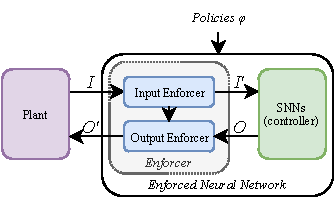
\includegraphics[width = \textwidth]{Content/fig/model-driven-ai-enns.pdf}
	\caption{Architecture of an enforced neural network}
	\label{fig:rebasic}
\end{figure}

\ignore{
\begin{figure}[!htb]
	\centering
	\begin{tikzpicture}[->, >=stealth', shorten >=0.15mm, shorten <=0.15mm, semithick, scale=0.8, transform shape]

\def\separation{20mm}

\tikzstyle{line} = [draw, -latex']

\tikzset{complete-box/.style={rectangle, draw, fill=none, minimum height=2.2cm, text width = 1.8cm, text centered}}

\tikzset{dashed-box/.style={complete-box, dashed, fill=black!10}}


\node[dashed-box]
(Plant) {$Plant$};

\node[complete-box, anchor=west] at ($ (Plant.east) + (\separation, 0) $)
(Enforcer) {$Enforcer$};

\node[dashed-box, anchor=west] at ($ (Enforcer.east) + (\separation, 0) $)
(Controller) {$Controller$};

\node [above = 0.25*\separation of Enforcer.north] (prop) {$\varphi$};


\node [anchor=south] at ($ (Plant.north east) + (0.5*\separation, 0.125*\separation) $) (inputsLabel) {Inputs};

\node [anchor=south] at ($ (Enforcer.north east) + (0.5*\separation, 0.125*\separation) $) (transformedInputsLabel) {Transformed Inputs};

\node [anchor=north] at ($ (Enforcer.south east) + (0.5*\separation, -0.125*\separation) $) (outputsLabel) {Outputs};

\node [anchor=north] at ($ (Plant.south east) + (0.5*\separation, -0.125*\separation) $) (transformedOuputsLabel) {Transformed Outputs};


\draw[->] (Plant.40) -- node[above] { \small $A$ } (Enforcer.140);
\draw[->] (Plant.20) -- node[above] { \small $B$ } (Enforcer.160);
\draw[->] (Enforcer.200) -- node[above] { \small $C'$ } (Plant.340);
\draw[->] (Enforcer.220) -- node[above] { \small $D'$ } (Plant.320);

\draw[->] (Enforcer.40) -- node[above] { \small $A'$ } (Controller.140);
\draw[->] (Enforcer.20) -- node[above] { \small $B'$ } (Controller.160);
\draw[->] (Controller.200) -- node[above] { \small $C$ } (Enforcer.340);
\draw[->] (Controller.220) -- node[above] { \small $D$ } (Enforcer.320);

\draw[->] (prop.south) -- (Enforcer.north);


\end{tikzpicture}

	\caption{Architecture of an enforced neural network}
	\label{fig:rebasic2}
\end{figure}
}

%\subsection{Synchronous Neural Networks}


%\subsection{Meta Neural Networks}

\subsection{Methodology and Assumptions}

The design of \acp{ENN} is performed as follows. The Esterel~\cite{Berry00}
synchronous programming language is used for the implementation of
\acp{SNN}. We can use existing C-based libraries such as
Darknet~\cite{darknet13} to create neural networks during the learning
phase. Once the learning phase is completed, we can create C-functions
with associated header files which store the weights. These can then be
invoked as \texttt{host-functions} in Esterel to create an individual \ac{SNN}. 

Esterel also provides an excellent avenue to create complex
applications using  \emph{synchronous concurrency}. This enables
several \acp{SNN} to be composed synchronously to
create neural network ensembles~\cite{Maqsood2004}, which are very useful in
creating complex AI applications that combine \acp{CNN} with other
types of \acp{ANN} in a systematic way. 

A given ensemble becomes a synchronous program, which can be combined
with other synchronous components easily in Esterel as the composition
of synchronous modules. We use this to combine the controller
represented as a neural network ensemble with the enforcer. Finally,
the overall system is composed with the reactive environment using the
standard approach of reactive interfaces. As Esterel programs are
automatically compiled to a single reactive function in C, where all
concurrency is ``compiled away'', the generated code is WCET
analysable, as shown in~\cite{sann}. However, this part is outside the
scope of the current work.